\section{Limitaciones conocidas de los LLM}
\label{sec:limitaciones_llm}
Ventana de contexto, sesgos, alucinaciones, dar la razón al usuario, 

Seguimos a \cite{arunbijiRAGVsFinetuning}



\subsection{Corte de conocimiento}

Los \gls{llm} no aprenden nuevos datos tras su entrenamiento, por lo que existe una limitación en la información o el conocimiento disponible al no haber tenido acceso a información o acontecimientos ocurridos después de esa fecha límite. Esta limitación se minimiza con rentrenamientos tipo \textit{fine-tuning} o con técnicas como \gls{rag}.

\subsection{Alucinaciones}

La finalidad de un \gls{llm} es <<modelar>> el lenguaje humano, con lo que, a priori, no se puede esperar que los datos que de en sus respuestas sean ciertos sino verosímiles. Los \gls{llm} se entrenan con vastas cantidades de datos de diversa calidad, y la trazabilidad de los datos que devuelve en sus respuestas es muy difícil de determinar. Precisamente, la técnica \gls{rag} permite dibujar la trazabilidad de los datos de las respuestas, en tanto en cuanto estas se basan en los datos de la base de datos de conocimiento. Por otra parte, la constante mejora de los datos de entramiento de los \gls{llm} \citep{gunasekarTextbooksAreAll2023} hace que este problema se minimice aunque nunca se elimina completamente.

\subsection{Ineficiencia y coste}

Una de las razones por las que los \gls{llm}, y toda la \gls{ia} generativa en general, no se ha desarrollado hasta hace relativamente poco tiempo, es la alta demanda de recursos computacionales que requiere tanto su fase de entrenamiento como su fase de inferencia. La carrera actual en el desarrollo de la \gls{ia} reside en ganar eficiencia en los modelos. 

Los problemas de eficiencia y coste se pueden articular en torno a tres ejes \citep{arunbijiRAGVsFinetuning}:

\begin{enumerate}[label=\alph*)]
    \item \textbf{Recursos de tiempo computacional:} El tiempo necesario para entrenar un \gls{llm} es muy alto, y depende del tamaño del modelo, del conjunto de datos de entrenamiento y de la capacidad de cómputo disponible. En general, se habla en términos de <<años de GPU>>, lo cual está fuera del alcance de la computación de usuario. La Figura \ref{fig:llm_gpu_training_hours} muestra el coste en millones de horas de GPU de diversos modelos de lenguaje de código abierto. En la fase de inferencia el coste computacional, aunque menor que en la fase de entrenamiento, sigue siendo alto, lo cual constituye un problema para el uso de \gls{llm} en local en dispositivos de usuario final.
    \item \textbf{Recursos de memoria:} Pero no es el tiempo de procesador el único origen de la ineficiencia. Estos modelos, de tamaños gigantescos, requieren de grandes cantidades de memoria RAM para su entrenamiento e inferencia. En \gls{llm} \textit{open source} como Mistral o Llama, en versiones comparables en rendimiento a GPT-3.5, se necesita entre 16 y 100 GB en GPU para la inferencia. 
    \item \textbf{Recursos económicos:} Finalmente, los costes computacionales se traducen en costes económicos, solo asumibles por grandes empresas. De ahí que la mayoría de \gls{llm} sean propiedad de grandes empresas como Google, Facebook o Microsoft, quienes los ponen a disposición de los usuarios a través de sus API.
\end{enumerate}

\begin{figure}[H]
    \caption[Coste de entrenamiento en horas de GPU de diversos modelos de lenguaje]{Coste de entrenamiento en horas de GPU de diversos modelos de lenguaje.}
    \centering
    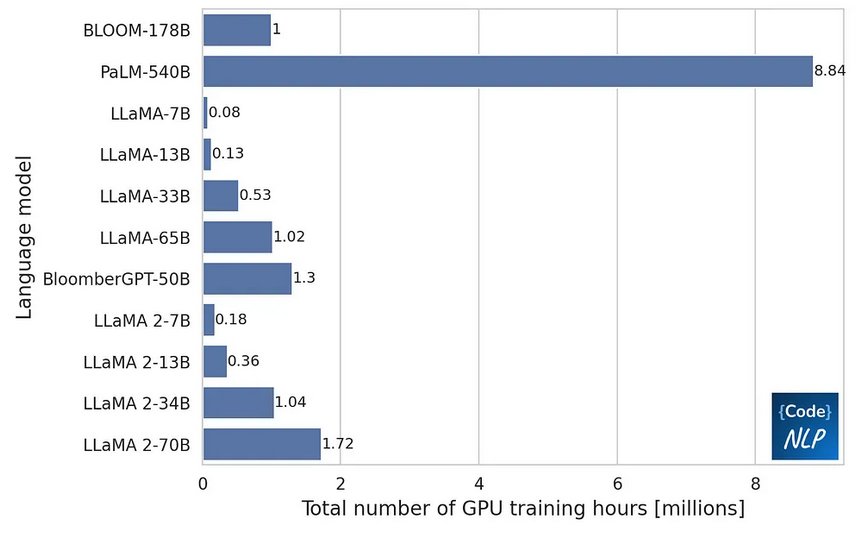
\includegraphics[width=0.8\textwidth]{./figuras/llm_gpu_training_hours.png}
    \source{\cite{ph.dTrainingTimeFoundation2023}}
    \label{fig:llm_gpu_training_hours}
  \end{figure}

Es de esperar que la eficiencia de recursos mejore con el tiempo. De hecho, ya se están viendo significativos avences en este sentido, especialmente de la mano del \textit{open source}, que está democratizando el acceso a los \gls{llm} y a la \gls{ia} en general, con sus contribuciones a mejoras en la arquitectura de los modelos, su proceso de entrenamiento, la eficiencia en dispositivos de bajos recursos y la creación de conjutos de datos de entreamiento de alta calidad, entre otros. En estos momentos, la gran mayoría de modelos de código abierto que grandes empresas crean y entrenan, y los propios usuarios rentrenan con un \textit{fine-tuning}, se pueden descargar y utilizar de forma gratuita en webs como \href{https://huggingface.co/}{Hugging Face}.


\subsection{Modelos de <<caja negra>>, con sesgos y riesgos}

Los \gls{llm} son modelos <<caja negra>>, es decir, no se puede conocer el proceso interno que sigue el modelo para generar sus respuestas. Esto es así porque los \gls{llm} son modelos estadísticos, y su funcionamiento se basa en la probabilidad de que un \textit{token} siga a otro. Por tanto, no se puede conocer el proceso interno que sigue el modelo para generar sus respuestas. Esto es especialmente importante en el caso de los \gls{llm} porque, a diferencia de otros modelos de \gls{ia}, como los modelos de clasificación, los \gls{llm} no se entrenan con datos etiquetados, sino que aprenden de forma autónoma a partir de grandes cantidades de datos sin etiquetar.

La opacidad de los \gls{llm} es un problema porque, al no conocerse el proceso interno que sigue el modelo para generar sus respuestas, no se puede conocer el sesgo que pueda tener el modelo. Un sesgo es una tendencia o inclinación a favor o en contra de algo o alguien, que generalmente se considera injusta. En el caso de los \gls{llm}, el sesgo se refiere a la tendencia a generar respuestas que favorezcan a un grupo o colectivo en detrimento de otro. Por ejemplo, un \gls{llm} entrenado con textos de Internet puede tener sesgos de género, raza, religión, etc. que se reflejen en sus respuestas.

Estos problemas de opacidad y de sesgo constituyen un potencial riesgo de seguridad, además de un problema ético. Aunque las grandes empresas implicadas en el desarrollo de modelos generativos de \gls{ia} están trabajando en minimizar estos problemas, es importante tener conciencia de ellos y de sus posibles consecuencias, independientemente de la finalidad con la que se utilicen los modelos.